\documentclass[a4paper,12pt]{article}
\usepackage[utf8]{inputenc}
\usepackage{amsmath}
\usepackage{graphicx}
\usepackage{caption}
\usepackage{enumitem}
\usepackage{float}

\title{5. röpdolgozat (6. gyakorlaton)}
\author{}
\date{}

\begin{document}

\maketitle

\begin{enumerate}

\item \textbf{Milyen ekvivalens átfogalmazást ismer a pontbeli deriválhatóságra a lineáris közelítéssel?}
    \begin{figure}[H]
        \centering
        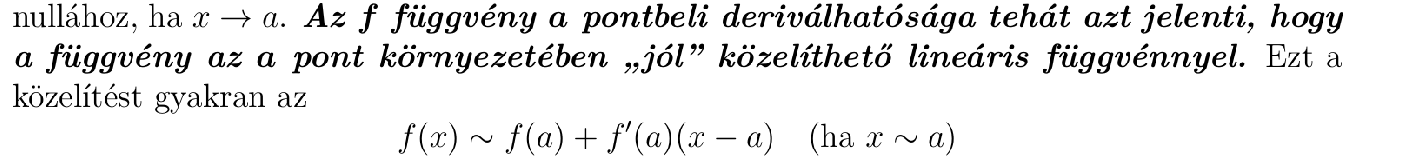
\includegraphics[width=0.8\textwidth]{gyak6answers/1.png}
        \caption{Válasz az 1. kérdésre}
    \end{figure}

\item \textbf{Mi a Taylor-polinom definíciója?}
    \begin{figure}[H]
        \centering
        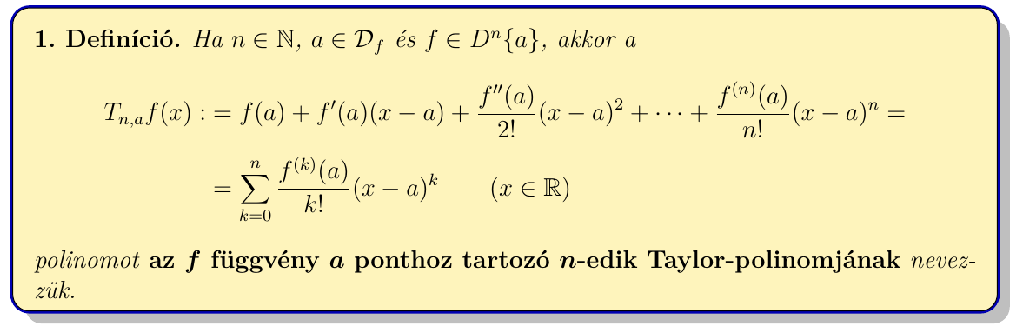
\includegraphics[width=0.8\textwidth]{gyak6answers/2.png}
        \caption{Válasz a 2. kérdésre}
    \end{figure}

\item \textbf{Mi a kapcsolat a függvénynek és Taylor-polinomjának deriváltjai között a Taylor-polinom középpontjában?}
    \begin{figure}[H]
        \centering
        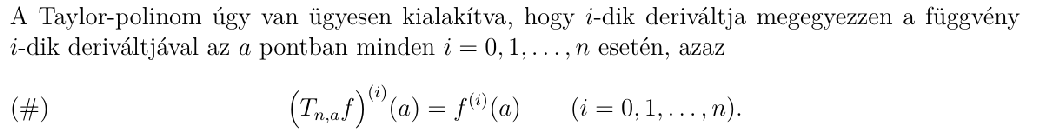
\includegraphics[width=0.8\textwidth]{gyak6answers/3.png}
        \caption{Válasz a 3. kérdésre}
    \end{figure}

\item \textbf{Fogalmazza meg a \textit{Taylor-formula a Lagrange-féle maradéktaggal} néven tanult tételt!}
    \begin{figure}[H]
        \centering
        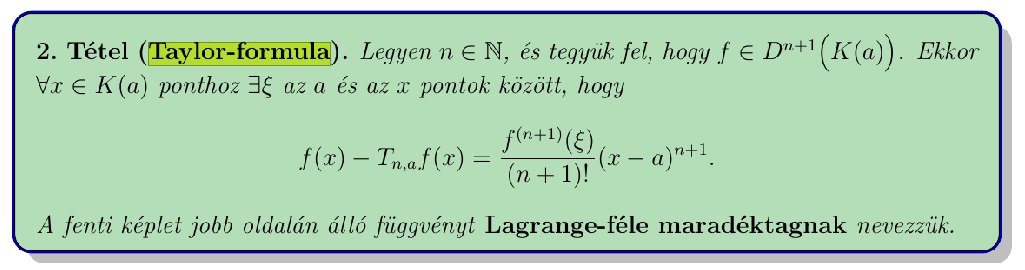
\includegraphics[width=0.8\textwidth]{gyak6answers/4.png}
        \caption{Válasz a 4. kérdésre}
    \end{figure}

\item \textbf{Hogyan definiálja egy függvény Taylor-sorát?}
    \begin{figure}[H]
        \centering
        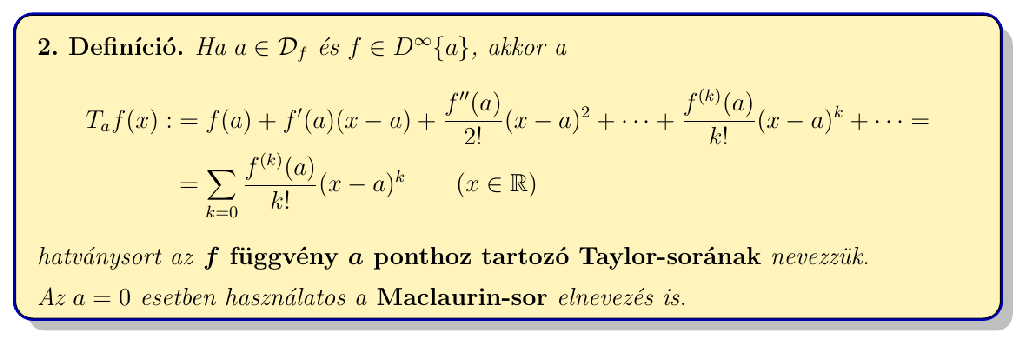
\includegraphics[width=0.8\textwidth]{gyak6answers/5.png}
        \caption{Válasz az 5. kérdésre}
    \end{figure}

\item \textbf{Mi a kapcsolat hatványsor összegfüggvényének a deriváltjai és a hatványsor együtthatói között?}
    \begin{figure}[H]
        \centering
        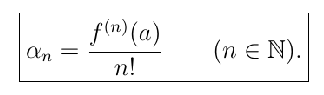
\includegraphics[width=0.8\textwidth]{gyak6answers/6.png}
        \caption{Válasz a 6. kérdésre}
    \end{figure}

\item \textbf{Milyen elégséges feltételeket ismer függvények Taylor-sorral történő előállítására?}
    \begin{figure}[H]
        \centering
        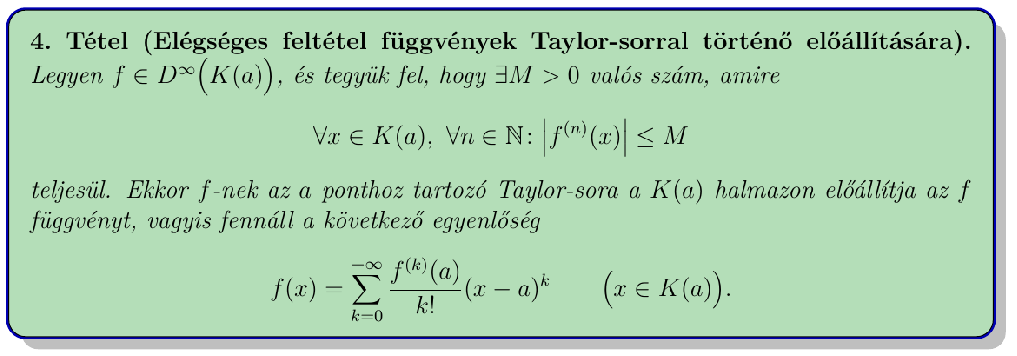
\includegraphics[width=0.8\textwidth]{gyak6answers/7.png}
        \caption{Válasz a 7. kérdésre}
    \end{figure}

\item \textbf{Milyen állítást ismer az $\frac{1}{1-x}$ függvény hatványsoros előállítására?}
    \begin{figure}[H]
        \centering
        \includegraphics[width=0.8\textwidth]{gyak6answers/8.png}
        \caption{Válasz a 8. kérdésre}
    \end{figure}

\item \textbf{Milyen állítást ismer az ln(1 + x) függvény hatványsoros előállítására?}
    \begin{figure}[H]
        \centering
        \includegraphics[width=0.8\textwidth]{gyak6answers/9.png}
        \caption{Válasz a 9. kérdésre}
    \end{figure}

\item \textbf{Milyen állítást ismer az arc tg függvény hatványsoros előállítására?}
    \begin{figure}[H]
        \centering
        \includegraphics[width=0.8\textwidth]{gyak6answers/10.png}
        \caption{Válasz a 10. kérdésre}
    \end{figure}

\end{enumerate}



\end{document}


